
\newpage

\begin{tikzpicture}[remember picture,overlay]
  \begin{scope}[on background layer]
    \node[anchor=north west,outer sep=0,inner sep=0] (img) at (current page.north west) {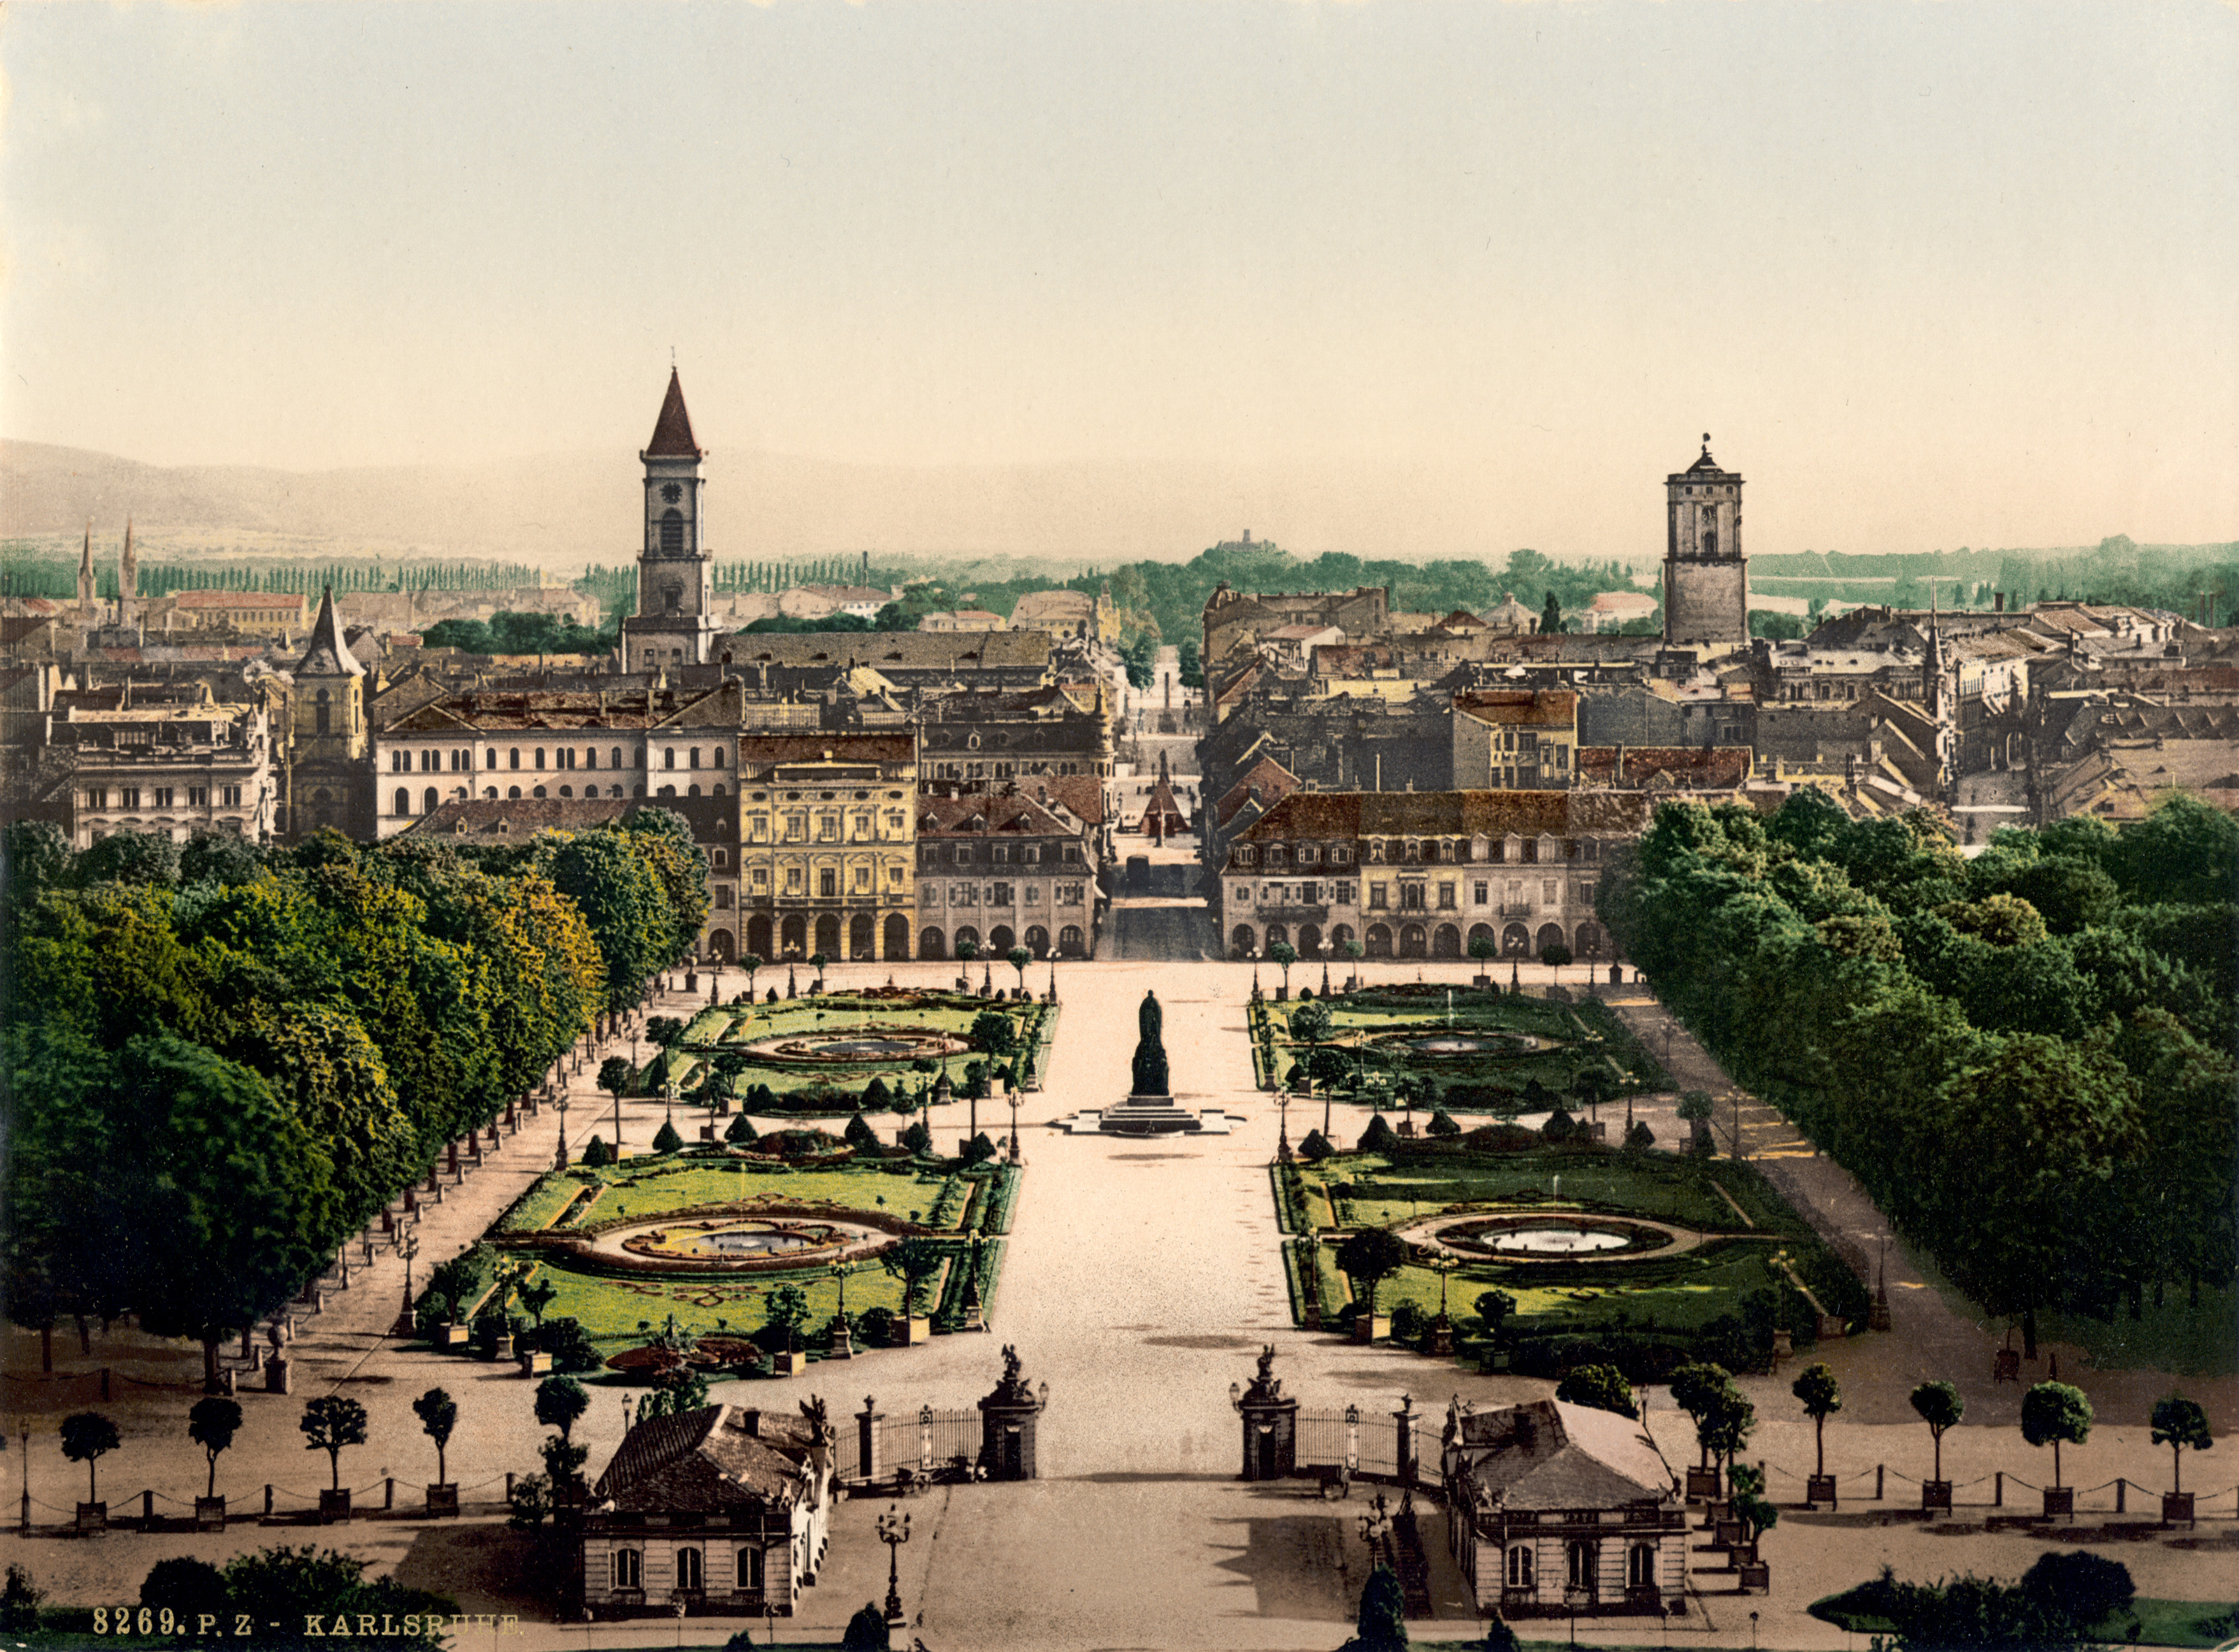
\includegraphics[width=21cm,trim=0 20 0 500,clip]{images/city/city-historic-1.jpg}};
  \end{scope}
  \node[anchor=south west,color=black,xshift=1ex,yshift=1ex] (label) at (img.south west) {\imgtitle{Library of Congress}{Karlsruhe between ca. 1890 and ca. 1900}{public domain, LC-DIG-ppmsca-00315, \url{http://lccn.loc.gov/2002713591}}};
  \begin{scope}[on background layer]
    \node[fit=(label),inner sep=0,outer sep=0,opacity=0.6,fill=white,rounded corners] {};
  \end{scope}
\end{tikzpicture}

\vspace*{8.2cm}


\section{Dining}

\subsection{Breakfast}
There are little German bakeries all over the city where you can get breakfast (savoury or sweet pastries and coffee or tea) for about \SI{4}{\euro}. However, breakfast is included in room fares at the Ibis hotel and A\&O, as well B\&B have common dining rooms and kitchen where everyone can prepare their usual breakfast.
 
\subsection{Lunch}
The university canteen offers meals for about \SI{3}{\euro} for students and \SI{6}{\euro} for guests. Otherwise, all type of restaurants (Kebabs, Thai, Chinese, Italian, …) are available all over the inner city. If one knows where to go it is possible to get a simple meal including drink for \SI{6}{\euro}.


\subsection{Dinner}

We intend to organize a picnic in the “Schlosspark” as well as a BBQ. We are not
currently planning on providing dinner for the other days, but there are a lot
of restaurants in the city with reasonably priced food. Expect meals to cost
around \SI{10}{\euro} without a drink, but there are also cheaper options for
as low as \SI{6}{\euro} including a drink available.

%As you can see, accessibility of the location, prices of accommodation and
%meals, as well as the overall concept elaborated by the organizing committee
%are all speaking in favor of hosting GUADEC in August 2016 in the sunny city
%of Karlsruhe! We are looking forward to welcoming you!

